\begin{wrapfigure}[9]{r}[0cm]{2.66cm}
	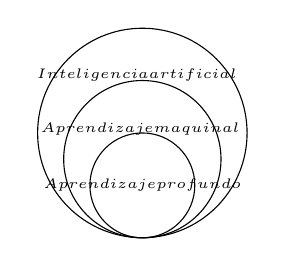
\begin{tikzpicture}
	\def\IA{(0,0) circle (1.33cm)}
	\def\AM{(270:.333cm) circle (.999cm)}
	\def\AP{(270:.666cm) circle (.666cm)}
	\draw \IA node[above]{\tiny$^{^{^{^{^{^{^{^{\overunderset{\text{ Inteligencia}}{\text{ artificial}}{}}}}}}}}}$};
	\draw \AM node[above]{\tiny$^{^{^{\overunderset{\text{Aprendizaje}}{\text{maquinal}}{}}}}$};
	\draw \AP node{\tiny$\overunderset{\text{Aprendizaje}}{\text{profundo}}{}$};
\end{tikzpicture}\caption[Inteligencia artificial]{\\Inteligencia\\artificial}\label{FIG:IA}
\end{wrapfigure}\subsection {Inteligencia artificial}\label{subsec:intela}
La \emph{ingeligencia artificial es}
\begin{displayquote}
el esfuerzo por automatizar tareas intelectuales normalmente realizadas por humanos(\citeauthor{cho18}, \citeyear{cho18})
\end{displayquote}
\begin{displayquote}
``es una de las disciplinas más sofisticadas creadas por el ser humano (...) está permitiendo obtener resultados similares a los que observamos en las capacidades de la inteligencia humana: reconocimiento del entorno y percepción espacial, predicción y anticipación, entendimiento del lenguaje y capacidades de comunicación...'' recordar cómo citar entrevistas en páginas web www.apd.es/ entrevista-gfi-estamos-asistiendo -al-auge-de -agentes-inteligentes-capaces-de-comunicarse -como-una-persona\end{displayquote}
de este campo general se desprenden el \emph{aprendizaje maquinal} y el \emph{aprendizaje profundo}, figura (\ref{FIG:IA}).

Dentro de los múltiples tipos de inteligencia artificial, los que son de nuestro interés para este proyecto se describen a continuación.\\

Aprendizaje maquinal\\
Burkov (\citeyear{burk19}) lo define como
\begin{displayquote}
preocupado con construir algoritmos que, para ser útiles dependen de una colección de ejemplos de algún fenómeno (...) el proceso de resolver problemas prácticos por 1) reunir un conjunto de datos y, 2) construir algorítmicamente un modelo estadístico basado en ese conjunto de datos
\end{displayquote}

A diferencia del paradigma clásico de programación, donde los humanos introducen órdenes y datos para ser procesados de acuerdo con dichas reglas, en el aprendizaje maquinal el humano introduce datos y respuestas esperadas de estos datos como ejemplos, el resultado es la generalización de ciertas respuestas a partir de dichos datos sin estructurar. Con ello, se induce al conocimiento por parte de la computadora.\\

%Si un sistema no es programado explícitamente, entonces se puede considerar una modalidad de aprendizaje maquinal como entrenamiento, tal que se le presentan muchos ejemplos relevantes a una tarea, y si encuentra una estructura estadística en ellos, genera reglas para automatizar la tarea.

Lingüística computacional\\
Es un campo multidisciplinario de la lingüística aplicada en la informática. Se sirve de los sistemas informáticos para el estudio y el tratamiento del lenguaje. Para ello, se intenta modelar de manera lógica el lenguaje natural desde un punto de vista programable.\\

Procesamiento del lenguaje natural\\
Es una disciplina de la rama de la ingeniería para la lingüística computacional. Se utiliza para la formulación e investigación de mecanismos de eficacia informática para servicios de comunicación entre las personas o entre ellas y las máquinas usando lenguajes naturales. Dos de los módulos básicos de procesamiento natural del lenguaje son búsqueda y aprendizaje con los que se pueden resolver muchos problemas con técnicas de optimización enfocadas en los diferentes parámetros involucrados.